\section{Vertical Shifting}

Very similar to the horizontal position change, the vertical position change
merely requires the transformation matrix to be shifted row-wise as opposed
to
column-wise.
\[
  \underbrace{
    \begin{bmatrix}
      1&0&0\\
      0&1&0\\
      0&0&1\\
    \end{bmatrix}
  }_{\text{Identity Matrix}}
  \implies
  \underbrace{
    \begin{bmatrix}
      0&0&1\\
      1&0&0\\
      0&1&0\\
    \end{bmatrix}
  }_{\text{Transformation
  Matrix}}
\]
Unlike the horizontal matrix shift, the order by which the transformation
matrix is applied is reversed:
\[ 
  \begin{bmatrix}
    a&b&c\\
    d&e&f\\
    g&h&i\\
  \end{bmatrix}
  \cdot
  \begin{bmatrix}
    0&0&1\\
    1&0&0\\
    0&1&0\\
  \end{bmatrix}
  =
  \underbrace{
    \begin{bmatrix}
    g&h&i\\
    a&b&c\\
    d&e&f\\
    \end{bmatrix}
  }_{\text{The
    vertically
    shifted
  matrix}}
\]

\begin{figure}[ht]
  \centering
  \begin{subfigure}{\textwidth}
    \centering
    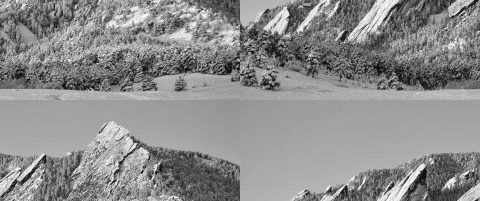
\includegraphics[scale=0.4]{./img/vhsg1.png}
    \caption{Photo 1 - Vertical and
    Horizontal Shift}
    \label{fig:p1vg}
  \end{subfigure}
  \begin{subfigure}{\textwidth}
    \centering
    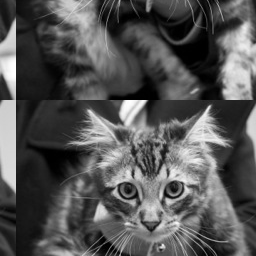
\includegraphics[scale=0.4]{./img/vhsg2.png}
    \caption{Photo
      2
      -
      Vertital
      and
      Horizontal
    Shift}
    \label{fig:p2vg}
  \end{subfigure}
  \caption{Vertically
    Shifted
  Images}
  \label{fig:vs_images}
\end{figure}

We can do both horizontal and vertical translations on our image matrix, but we must do the operations separately for photo1.jpg since they do not involve the same number of iterations. For example, we can first do the horizontal translation by using the same procedure above where the transformation matrix is second in the matrix multiplication (the transformation matrix would be dimension $n \times n$, where “$n$” equals the column dimension of photo1.jpg, 408). After performing the 240 iterations of this horizontal translation we can then translate the image matrix vertically. We now place the transformation matrix first in the matrix multiplication; its dimensions must match the row dimension of the image. Therefore, this vertical transformation matrix is $201\times 201$.
